\section{\label{sec:clas.acc}Electron Accelerator}

The \abbr{CEBAF} electron accelerator is able to deliver a 75\% polarized electron beam of up to approximately 6~GeV to each of the three halls simultaneously. The beam as seen by each hall consists of clusters of electrons separated by approximately 2~ns. Typical intensities for halls \desg{A} and \desg{C} are 10--100~\text{$\mu$} A, however, due to the nature and sensitivity of the \abbr{CLAS} detector, beam currents to hall \desg{B} are typically 10--100~nA.

Using a GaAs photocathode laser driven gun system, a highly polarized electron beam is produced and accelerated through a radio-frequency (\abbr{RF}) chopping system operating at 499~MHz. The three-beam, 1497~MHz ``bunch train'' at 100~keV is then longitudinally compressed and accelerated to just over 1\% of the total machine energy before it is injected into the first main accelerator. This compression results in a beam of 2~ps bunches separated by 668~ps.

The main accelerator consists of a pair of linear accelerators (\abbr{LINAC}s\label{abbr:linac}) which consists of twenty cryomodules each containing eight superconducting niobium cavities as shown in Fig.~\ref{fig:jlab.cavity}. This was the first use of superconducting cavities and marked a major advancement in the field of accelerators. Prior to the \abbr{CEBAF} breakthrough, typical accelerating cavities used non-superconducting metals like copper whose resistivity would cause a build up of heat. The niobium superconducting cavities are kept at 2~Kelvin and are non-resistive, eliminating the heating problems of copper. The significant cooling requirements are satisfied by the Lab's Central Helium Liquefier (\abbr{CHL}\label{abbr:chl}).

\begin{figure}\begin{center} 
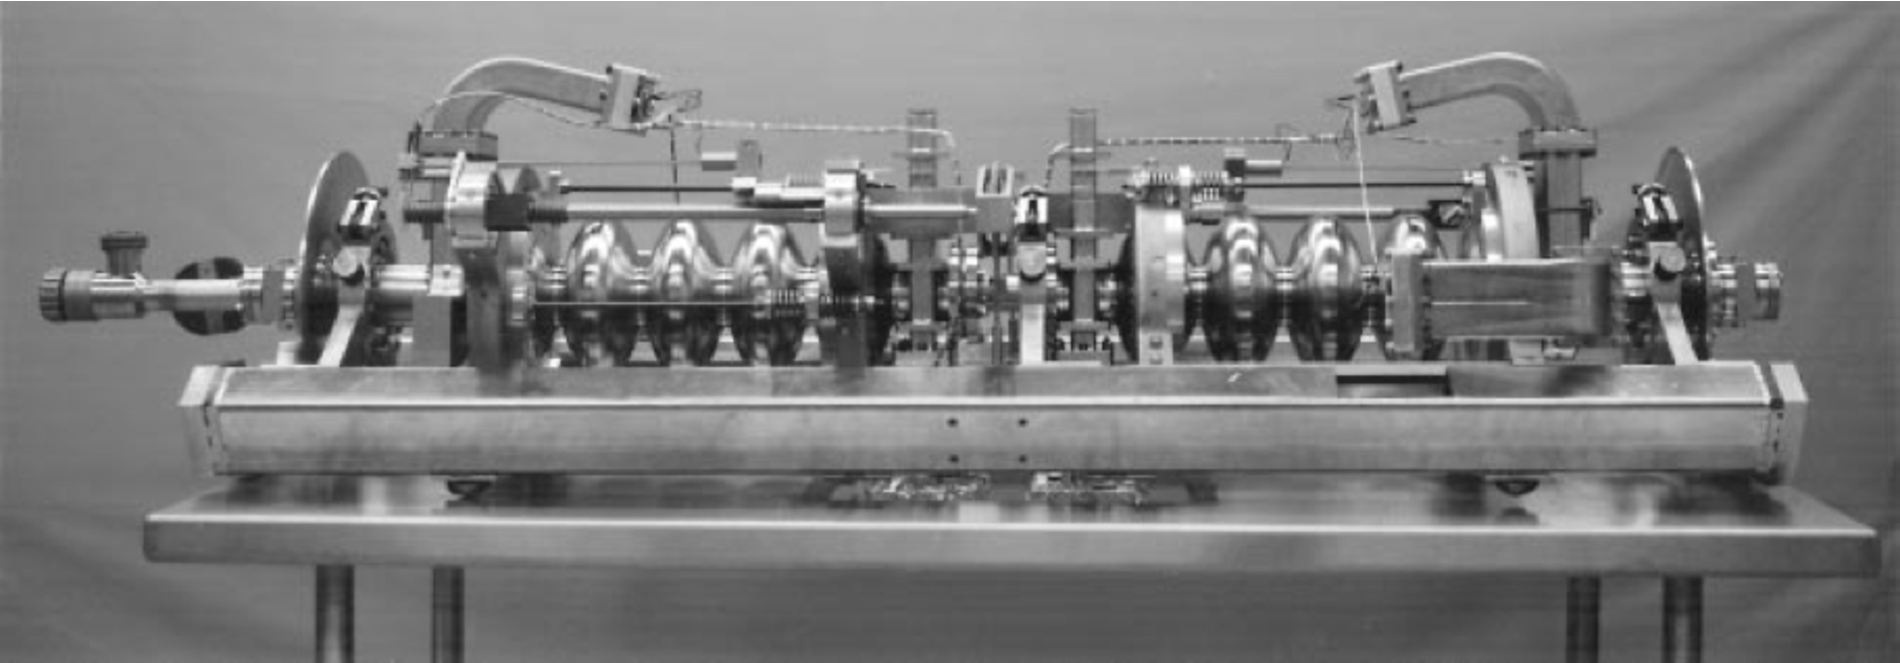
\includegraphics[width=\figwidth]{\grpath/jlab/niobium_cavity_pair.pdf}
\caption[Niobium Cavity Pair (photograph)]{\label{fig:jlab.cavity}A superconducting niobium cavity pair. These devices are tuned for specific energy resonances by mechanically adjusting their lengths on the order of a few micrometers.}
\end{center}\end{figure}

A standing electromagnetic wave is induced inside the niobium cavities as shown in Fig.~\ref{fig:jlab.accel} and the electrons passing through experience a continuous acceleration. Before \abbr{CEBAF}, the copper accelerating cavities used were tuned by adjusting the cooling system. The resistivity of the copper would cause the cavity to heat up and expand and the cooling system would be set so the desired length was obtained. The superconducting niobium cavities on the other hand are non-resistive and do not heat up. Therefore, the cavities are lengthened or shortened mechanically (on the order of a few micrometers) to tune the wavelength and maximize the acceleration of the electrons.

\begin{figure}\begin{center}
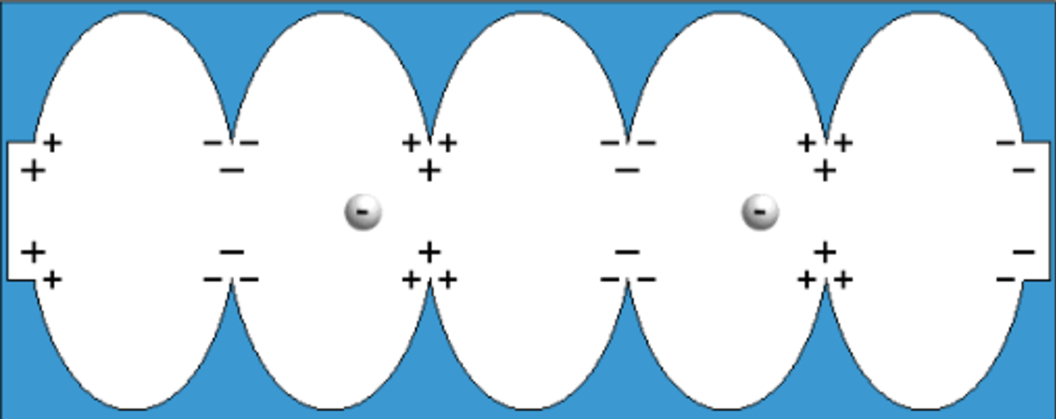
\includegraphics[width=0.8\figwidth]{\grpath/jlab/accelerating_diagram.pdf}
\caption[Accelerating Cavity Diagram]{\label{fig:jlab.accel}As the electron clusters travel through a superconducting niobium cavity, shown in Fig.~\ref{fig:jlab.cavity}, they experience a continuous acceleration due to a standing electromagnetic wave indicated by the positive and negative signs along the inner wall.}
\end{center}\end{figure}

The \abbr{LINAC}s are connected by two sets of 180$^\circ$ magnetic-dipole bending arcs (see Fig.~\ref{fig:jlab.cebaf}) with a radius of 80~meters. The beam is sent through both accelerators and is then \emph{recirculated} up to four more times. Each \abbr{LINAC} is capable of accelerating the beam by up to 600~MeV giving approximately 1.2~GeV per pass. A plan to nearly double the energy of the beam was approved by \abbr{DOE}\label{abbr:doe} and the 12~GeV program started construction on September 15, 2008\cite{jlab.news.cd3, jlab.12gev.starts}.

The beam is selectively extracted using \abbr{RF} cavities tuned to 499~MHz --- the frequency dictated by the manufactured geometry. By slightly accelerating every third bunch, while not disturbing the other two, the electrons are bent out of the recirculating \abbr{LINAC} and sent to one of the halls. Each of the first four passes can be delivered to only one hall at a time, however the fifth (final) pass can be sent to all three halls simultaneously. The 499~MHz extraction creates the final beam as seen by the hall which consists of $\sim2$~ps bunches separated by 2.004~ns. At the time of the \g12 experiment, the accelerator was capable of delivering a maximum electron beam energy of 5.7~GeV. The tagger subsystem (see Sec.~\ref{sec:clas.tagr}) tagged photons of energies up to 95\% of the delivered beam, and therefore the maximum energy photon seen in \g12 was 5.4~GeV.
